% $File: report.tex
% $Date: Wed Jan 01 22:50:31 2014 +0800
% $Author: wyx <ppwwyyxxc@gmail.com>

\documentclass[11pt,a4paper]{article}
\usepackage{threeparttable}
\usepackage{dirtree}
\usepackage{keystroke}


\usepackage{fontspec,amsmath,amssymb,zhspacing,verbatim,minted,listings,zhmath}
\usepackage{titlesec, titletoc}
\usepackage{enumerate}
\usepackage[hyperfootnotes=false,colorlinks,linkcolor=blue,anchorcolor=blue,citecolor=blue]{hyperref}
\usepackage[backend=biber]{biblatex}
%\usepackage[dvips]{graphicx}
\usepackage{subfigure}
\usepackage{indentfirst}
\usepackage{float}			% don't automatically change location of figure [H]
\usepackage{chngpage}		% use \changetext to change page size
\usepackage{caption} \captionsetup{hypcap=true}  % ref to jump to object instead of caption
\newfontfamily\zhfont[BoldFont=SimHei,ItalicFont=KaiTi_GB2312]{SimSun}
\lstset{keywordstyle=\color{blue!70}, commentstyle=\color{red!50!green!50!blue!50},frame=shadowbox,rulesepcolor=\color{red!20!green!20!blue!20},
basicstyle=\footnotesize\ttfamily}
\zhspacing
\setlength{\parindent}{2em}

%use cell in tabular
\newcommand{\tabincell}[2]{\begin{tabular}{@{}#1@{}}#2\end{tabular}}

%thick shline
\newlength\savewidth
\newcommand\shline{\noalign{\global\savewidth\arrayrulewidth\global\arrayrulewidth 1pt}
                   \hline
                   \noalign{\global\arrayrulewidth\savewidth}}

\renewcommand{\abstractname}{摘要}
\renewcommand{\contentsname}{目录}
\renewcommand{\tablename}{表}
\renewcommand{\figurename}{图}
\defbibheading{bibliography}{\section{References}}
\bibliography{refs.bib}
\newcommand{\figref}[1]{\hyperref[fig:#1]{图\ref*{fig:#1}}}
\newcommand{\secref}[1]{\hyperref[sec:#1]{\ref*{sec:#1}节}}
\newcommand{\tabref}[1]{\hyperref[tab:#1]{表\ref*{tab:#1}}}

% math function
\let\Oldsum\sum
\renewcommand{\sum}{\displaystyle\Oldsum}
\let\Oldprod\prod
\renewcommand{\prod}{\displaystyle\Oldprod}

\usepackage{fancyhdr}
\changetext{}{2.2cm}{-1.1cm}{-1.1cm}{}
\pagestyle{fancy}
\setlength{\headheight}{15.2pt}
\lhead[]{}\rhead[]{}
\fancyhead[C]{\emph{FTP实验报告}}


\renewcommand{\baselinestretch}{1.2}

% $File: mint-defs.tex
% $Date: Fri Jan 06 14:25:30 2012 +0800
% $Author: wyx <ppwwyyxxc@gmail.com>


% \inputmintedConfigured[additional minted options]{lang}{file path}{
\newcommand{\inputmintedConfigured}[3][]{\inputminted[fontsize=\footnotesize,
	label=#3,linenos,frame=lines,framesep=0.8em,tabsize=4,#1]{#2}{#3}}

% \phpsrc[additional minted options]{file path}: show highlighted php source
\newcommand{\phpsrc}[2][]{\inputmintedConfigured[#1]{php}{#2}}
% \phpsrcpart[additional minted options]{file path}{first line}{last line}: show part of highlighted php source
\newcommand{\phpsrcpart}[4][]{\phpsrc[firstline=#3,firstnumber=#3,lastline=#4,#1]{#2}}
% \phpsrceg{example id}
\newcommand{\phpeg}[1]{\inputminted[startinline,
	firstline=2,lastline=2]{php}{res/php-src-eg/#1.php}}

\newcommand{\txtsrc}[2][]{\inputmintedConfigured[#1]{text}{#2}}
\newcommand{\txtsrcpart}[4][]{\txtsrc[firstline=#3,firstnumber=#3,lastline=#4,#1]{#2}}

\newcommand{\pysrc}[2][]{\inputmintedConfigured[#1]{py}{#2}}
\newcommand{\pysrcpart}[4][]{\pysrc[firstline=#3,firstnumber=#3,lastline=#4,#1]{#2}}

\newcommand{\confsrc}[2][]{\inputmintedConfigured[#1]{squidconf}{#2}}
\newcommand{\confsrcpart}[4][]{\confsrc[firstline=#3,firstnumber=#3,lastline=#4,#1]{#2}}

\newcommand{\cppsrc}[2][]{\inputmintedConfigured[#1]{cpp}{#2}}
\newcommand{\cppsrcpart}[4][]{\cppsrc[firstline=#3,firstnumber=#3,lastline=#4,#1]{#2}}


\title{FTP实验报告}
\author{吴育昕~2011011271\\(计14~ppwwyyxxc@gmail.com)}
\date{}

\begin{document}
%\fontsize{10pt}{\baselineskip}
%\selectfont
\maketitle

\titleformat*{\section}{\centering\Large\bf}
\tableofcontents



\section{实验目的}
文件传输是计算机网络的基本功能,文件传输协议(FTP)是一个基本的应用层
协议.本实验要求在Linux 系统上使用Socket 编程技术实现简化的FTP 服务器和客
户端的程序,使客户端可以连接至服务器,并且可以进行一些FTP 的基本操作,如
列出目录、下载文件等.

\section{实验原理}

FTP 是File Transfer Protocol,即文件传输协议的缩写.该协议用于在两台计算机
之间传送文件.基本模型如下:
\begin{figure}[H]
  \centering
  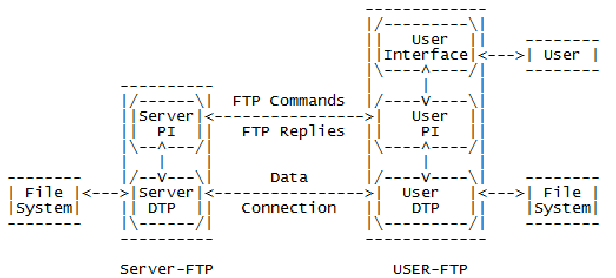
\includegraphics[width=\textwidth]{res/ftp1.png}
\end{figure}

FTP 会话包含两个TCP 连接通道,一个是控制通道,一个是数据通道.如下图
所示:
\begin{figure}[H]
  \centering
  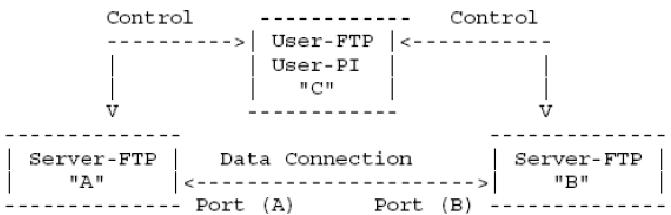
\includegraphics[width=\textwidth]{res/ftp2.png}
\end{figure}

控制通道是和FTP 服务器进行沟通的通道,连接FTP 服务器,发送FTP 指令;
数据通道则是和FTP 服务器进行文件传输或者获取文件列表的通道.
FTP 协议中控制连接的各种指令均由客户端主动发起,而数据连接有两种工作
方式:主动方式(PORT 方式)和被动方式(PASV 方式).主动方式下,FTP 客户
端首先和FTP 服务器的控制通道对应端口(一般为21)建立连接,通过控制通道发
送命令客户端需要接收数据的时候在这个通道上发送PORT 命令.PORT命令包含了
客户端用什么端口(一个大于1024 的端口)接收数据.在传输数据的时候,FTP 服
务器必须和客户端建立一个新的连接,服务器通过自己的TCP20端口发送数据.被
动方式下,建立控制通道的过程和主动方式类似,当客户端通过这个通道发送PASV
命令的时候, FTP server 打开一个位于1024$ \sim$5000 之间的随机端口并且通知客户端,
然后客户端与服务器之间将通过这个端口进行数据的传送.如下图所示:


\begin{figure}[H]
  \centering
  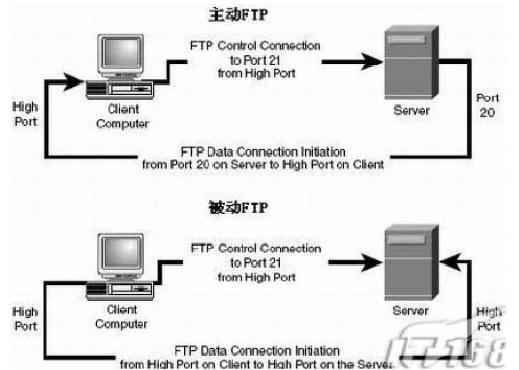
\includegraphics[width=0.8\textwidth]{res/ftp3.png}
\end{figure}


FTP 的工作流程如下:
\begin{enumerate}[(1)]
    \item FTP 服务器运行守护进程,等待FTP 请求.
    \item 它收到客户端的FTP 请求以后,建立控制连接,等待客户端命令.
    \item 如果服务器收到正确的传输文件命令,则新开一个数据连接,使用另外的端口进行传输.数据传输完以后,关闭数据连接.
    \item 如果服务器收到其他命令,则根据不同的命令做出响应.
    \item 如果收到quit 命令,结束控制连接,结束会话.
\end{enumerate}

%File: work.tex
%Date: Wed Jan 01 22:51:57 2014 +0800
%Author: Yuxin Wu <ppwwyyxxc@gmail.com>

\section{实验实现}
程序采用SugarCpp语言编写. SugarCpp是由我参与开发的一种可以翻译至C++的语言
\footnote{项目代码见\url{https://github.com/curimit/SugarCpp}}
, 它利用C++11标准为C++添加了语言特性与语法糖.

程序源代码见src目录, 翻译后的C++代码见cpp目录. 项目托管在github上. \footnote{\url{https://github.com/ppwwyyxx/SugarFTP}}

程序的Socket通信基于对TCP Socket的封装\verb|TCPSocket|类, 支持简单的发送/接收, 见\verb|Socket.sc|.
客户端与服务端对FTP命令的处理都通过CmdHandler类完成, 它管理了一个socket, 并利用它发送与接收FTP命令, 见\verb|Command.sc|.
客户端与服务端的实现分别位于\verb|Client.sc, Server.sc|

程序主要实现了以下功能:
\begin{enumerate}
  \item \verb|ls, cd, quit, rm, put, get, help|几条指令.

  \item 指令实现依照RFC959, 能够与FTP标准通信, 例如可以使用lftp\footnote{\url{http://lftp.yar.ru/}}, chrome对Server进行访问.

  \item 服务端多线程实现, 支持多个用户同时连接.

  \item 访问安全控制, 不允许访问根目录以外的路径.
\end{enumerate}

\subsection{客户端}
通过:
\begin{lstlisting}
$ ./client <host> <port>
\end{lstlisting}
运行客户端. 客户端成功与服务端建立连接后, 会使用anonymous用户登陆, 并使用\verb|TYPE I|以避免文件传输时换行符错误.

随后, 程序打印提示符``\verb|SugarFTP>|'', 可以输入命令. 对\verb|rm, cd|命令, 将其直接发送给服务端.
对\verb|get, put, ls|命令, 先进入PASV模式建立数据通道并获取端口, 再将其相应的发送给服务端后, 调用统一的接口\verb|Client::response()|获取返回数据.

\subsection{服务端}
用法:
\begin{lstlisting}
$ ./server <root dir> [port]
\end{lstlisting}

服务端的Socket一旦收到连接请求, 就利用\verb|std::thread|开启一个新的server worker线程, 进行会话.
会话由\verb|FtpSession|类管理, 负责处理各类命令.

服务端会对\verb|USER, TYPE, QUIT, FEAT, ALLO, PWD, PASV, LIST, CWD, RETR, STOR, SIZE|命令进行相应的处理.
其中, 对于文件及目录的访问, 做了权限限制, 所有根目录之外的文件都无法被客户端查看和下载.
对于文件访问中发生的各类错误, 如文件无法读取,无法写入等, 都会有相应的报错.



\section{思考题}
\begin{enumerate}

    \item 在FTP 协议中,为什么要建立两个TCP 连接来分别传送命令和数据?

    允许在传送数据的同时继续执行命令, 也允许了一个客户端可以同时传送几个数据.
    这些如果只有一个TCP连接, 实现起来将会有困难.


\item 主动方式和被动方式的主要区别是什么?为何要设计这两种方式?

两种模式发起连接的方向截然相反,主动模式是客户端规定端口,从服务器端向客
户端的这个端口发起连接; 被动模式是服务器告知客户端一个端口,客户端向服务
器端的这个端口发起连接.
设计这两种方式, 主要是为了避免服务器或客户端有一方无公网IP地址的情形(例如在NAT后),
用可选的这种方式, 只要有一方有公网IP, 就能正常建立数据连接.

\item 当使用FTP 下载大量小文件的时候,速度会很慢,这是什么缘故?可以怎样改进?

因为每传输一个文件,都要先建立连接,再传送数据,最后断开连接, overhead会很大.

\textbf{改进}: 连接保持一段时间后没有新的数据请求再断开.
\end{enumerate}

\section{总结}
这次实验加深了对FTP 协议一些细节方面的理解,熟练了Socket编程方法,同时也熟悉了POSIX底层API, 收获很大.
同时写出的FTP可与标准通信, 因而以后可以用于与别人快速交换数据, 也很有实用价值.

\printbibliography

\end{document}

